\section{Prüfung 02.02.2022}

\subsection{1. Echtzeit}
\subsubsection{a)}
Ein Profit/Penalty-Diagramm gibt den Nutzen bzw. den Schaden der Ausführung einer Operation als
kontinuierlichen Zahlenwert in Abhängigkeit vom Zeitpunkt der Ausführung an. Positive Werte
bedeuten einen Nutzen, negative einen Schaden – je größer der Absolutwert, desto größer der Nutzen
bzw. der Schaden.
Eine SPS mit einer Zykluszeit von 15 ms, einer Eingabezeit von 10 ms und einer Ausgabezeit von 5 ms
steuert eine Bremsanlage. Falls nach Betätigen des Bremshebels (als Sensor an die SPS angeschlossen)
mehr als 35 ms vergehen bis die Bremse (als Aktuator an die SPS angeschlossen) aktiviert wird, dann
kommt es zu einem Unfall. Die SPS wird zum Zeitpunkt 0 eingeschaltet, dann beginnt der erste EVADurchlauf und wiederholt sich dann periodisch alle 10+15+5=30 ms.
Zeichnen Sie in das Diagramm unten den Verlauf der Profit-Penalty-Funktion für die Operation
„Betätigen des Bremshebels“ ein.

\begin{figure}
  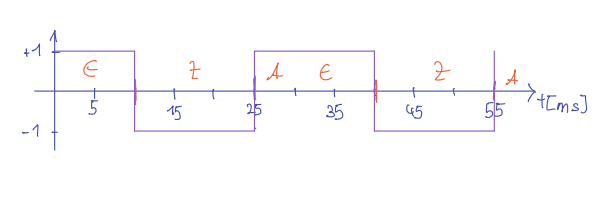
\includegraphics[width=10cm]{images/KA020222/1a.PNG}
  \centering
\end{figure}

\subsubsection{b)}
Handelt es sich hier um weiche, feste oder harte Echtzeit? Begründen Sie!

In diesem Beispiel handelt sich um harte Echtzeit. Wird der Bremshebel nicht betätigt wird es zu einem Schaden kommen.

\subsection{2. Echtzeitkommunikation}
\subsubsection{a)}
Nennen und erläutern Sie zwei wesentliche technische Unterschiede zwischen PROFInet SRT und
PROFInet IRT.

SRT = \textbf{S}oft \textbf{R}eal \textbf{T}ime wird für Prozess Automatisierung verwendet. Ist eine pure Software Lösung.
IRT = \textbf{I}sochronous \textbf{R}eal \textbf{T}ime wird für Motion Control verwendet. Ist eine Hardware Implementation  für Zyklus
synchronisation und Time slot control. Kleinere Zykluszeit und Jitter.

\subsubsection{b)}
Warum verwendet man bei Bluetooth „Frequency Hopping“?

Durch Frequency Hopping ist eine Übertragung unempfindlicher gegenüber Störungen sowie auch abhörsicher.

\subsubsection{c)}
Warum darf beim I²C-Bus der räumliche Abstand der Teilnehmer voneinander eine maximale
Distanz nicht überschreiten?

Überschreitet die räumliche Distanz zwischen den Teilnehmern einen bestimmten Wert kann es aufgrund der Abnahme
der Signalstärke zu Störungen oder Verlusten der Übertragung führen.

\subsubsection{d)}
Über einen CAN-Bus soll die Nutzdatenbitfolge „000000000010111“ übertragen werden. Geben Sie
die Bitfolge an welche daraus durch Bit-Stuffing entsteht.

Nach 5 bits wird ein Stuff-Bit eingefügt.
00000\textbf{1}00000\textbf{1}10111

\subsection{Echzeitscheduling}
Gegeben sind folgende drei Tasks:
Task1 = (1; 3)
Task2 = (1; 5)
Task3 = (1; 4)
Ein Task ist als Taskj=(Cj; Tj) definiert, wobei Cj die Ausführungszeit (Worst-Case) von Task j und Tj die
Periode von Task j ist. Wir benutzen das Task-Modell aus der Vorlesung, d.h. für jeden Task ist die Periode
identisch mit der Deadline, die Ausführungszeiten der Tasks sind konstant und so weiter. Alle Tasks sind
gleichzeitig zum Zeitpunkt 0 ausführungsbereit.

\subsubsection{a)}
Zeichnen Sie die Ausführung der drei Tasks gemäß RMS bis zum Zeitpunkt 20 in das Diagramm ein:

RMS = statisches Schedulingstrategie, zunehmende Taskperioden. Task mit kürzester Periode bekommt höchste Priorität
\begin{figure}
  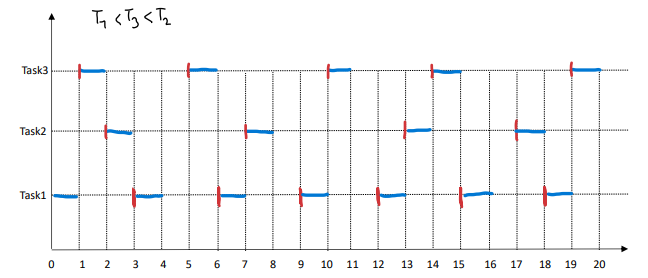
\includegraphics[width=10cm]{images/KA020222/2a.PNG}
  \centering
\end{figure}
\subsubsection{b)}
Werden die Deadlines aller Tasks bis in alle Ewigkeit eingehalten? Begründen Sie!

Nein werden sie nicht. Die Deadline von Task 3 kann schon bei Zeitschritt 9 nicht mehr eingehalten werden, da 
Task 1 diesen Slot besetzt. Der Task muss um 1 nach hinten verschoben werden. 

\subsection{Synchronisation}
Gegeben seien Tasks T1, T2 und T3, die Zugriff auf eine Ressource in einer bestimmten Reihenfolge
benötigen. Und zwar soll als erstes T1 Zugriff erhalten, danach sollen T2 und T3 gleichzeitig Zugriff erhalten.
Die Tasks sollen (eine oder mehrere) Semaphoren verwenden um dieses Zugriffsmuster zu garantieren.

\subsubsection{a)}
Zeichnen Sie in die untenstehenden Codegerüste die entsprechenden Semaphoren-Operationen ein
um das oben beschriebene Zugriffsmuster zu garantieren. Geben Sie bei jeder Operation an welche
Semaphore verwendet wird.
\begin{figure}
  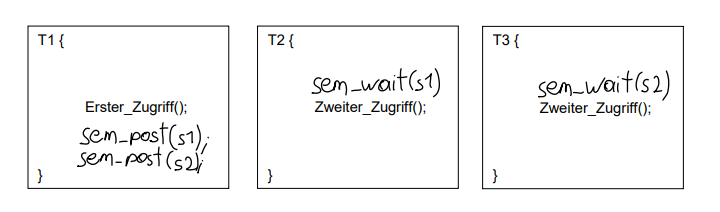
\includegraphics[width=10cm]{images/KA020222/4a.PNG}
  \centering
\end{figure}

\subsubsection{b)}
Geben Sie für jede verwendete Semaphore den initialen Wert an.

s1 und s2 werden mit 0 intialisiert, da sie bei T2 und T3 warten müssen bis T1 die Resource freigegeben hat.

\subsection{Statecharts}
Tragen Sie für den unten dargestellten Statechart in die folgende Tabelle jeweils alle aktiven (Sub)zustände
ein, die nach der Bearbeitung jedes der gegebenen Ereignisse aktiv sind. Die Ereignisse treten dabei
nacheinander ein, zuerst „a“, dann „d“, dann „a“, etc.

TODO ka.
\begin{figure}
  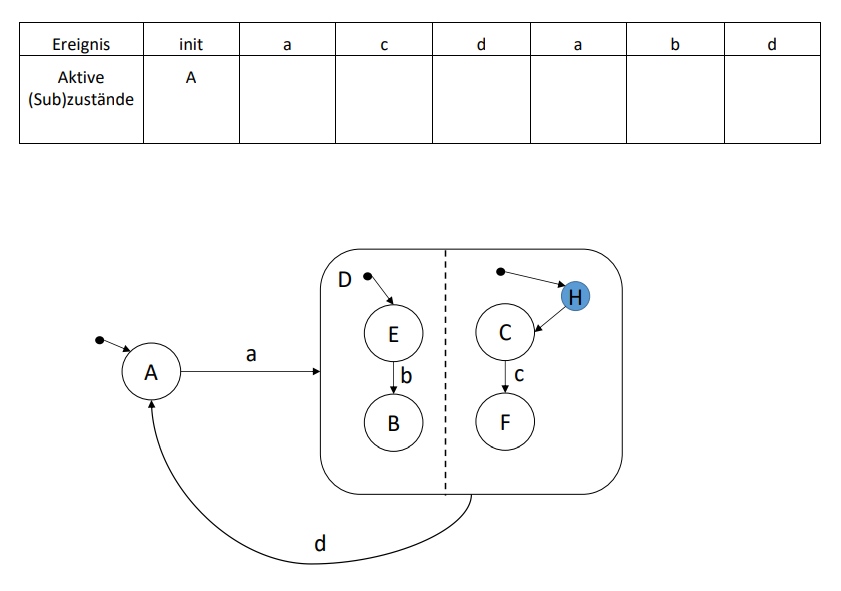
\includegraphics[width=10cm]{images/KA020222/5a.PNG}
  \centering
\end{figure}

\subsection{Speicherprogrammierbare Steuerung (SPS)}
\subsubsection{a)}
Warum werden die Sensorwerte zunächst in ein Eingabeabbildungsregister geladen anstatt die
Sensoren direkt im Steuerprogramm auszulesen?

Sensorwerte können dadurch synchronisiert und gefiltert werden, eine gleichmäßige Überwachung der Sensoren ist gewährleistet.

\subsubsection{b)}
Was versteht man unter der Reaktionszeit einer SPS und wie groß ist diese im besten Fall?

Maximale Response Time von Eingang zu Ausgang.
\begin{equation}
  t_r = t_i + 2t_c + t_o
\end{equation}
$t_i$ = input time, $t_c$ = cycle time, $t_o$ = output time
Im Idealfall wäre die Reaktionszeit 0.


\subsubsection{c)}
Kann man mit einer SPS auch eine Regelung implementieren? Begründen Sie warum bzw. warum
das nicht möglich ist.

Ja kann man. Regler haben meistens einen geschlossenen Regelkreis. Die SPS liest einen Wert, verarbeitet ihn,
gibt einen neuen Stellwert aus, und liest den neuen Istwert wieder ein und adaptiert wiederum den Stellwert.

\subsubsection{d)}
Gibt es Steuerungsaufgaben die mittels AWL beschrieben werden können jedoch nicht mit FUP?
Begründen Sie!

AWL ist eine sprachbasierte Programmiersprache, sie kann mit komplexen logischen Abläufen und Schaltalgorithmen umgehen.
Es sind spezielle Funktionen wie Interrupts, Timer und Datenverarbeitung möglich.

FUP ist eine graphische Programmiermethode. Für einfache logische Abläufe eignet es sich gut da logische Abläufe durch 
Verknüpfung von Funktionsblöcken dargestellt werden können. Keine umfassende Unterstützung für komplexe Algorithmen.